\chapter{ Questionários Utilizados na Avaliação Subjetiva}\label{apendice1}




% Texto ou documento elaborado pelo autor, a fim de complementar sua dissertação/argumentação.

Nesse anexo podem ser observados os questionários utilizados na Avaliação Subjetiva dos Extratores de Tópicos e segmentador (\textit{BayesSeg}) empregado nesse trabalho. 
O documento é composto por dois questionários sendo estes entregues a avaliadores divididos em dois grupos distintos.
A descrição completa desses questionários bem como as análises dos dados obtidos podem ser vistas nos Capítulos~\ref{cap-segmentadores}~e~\ref{cap-extratores}.

% 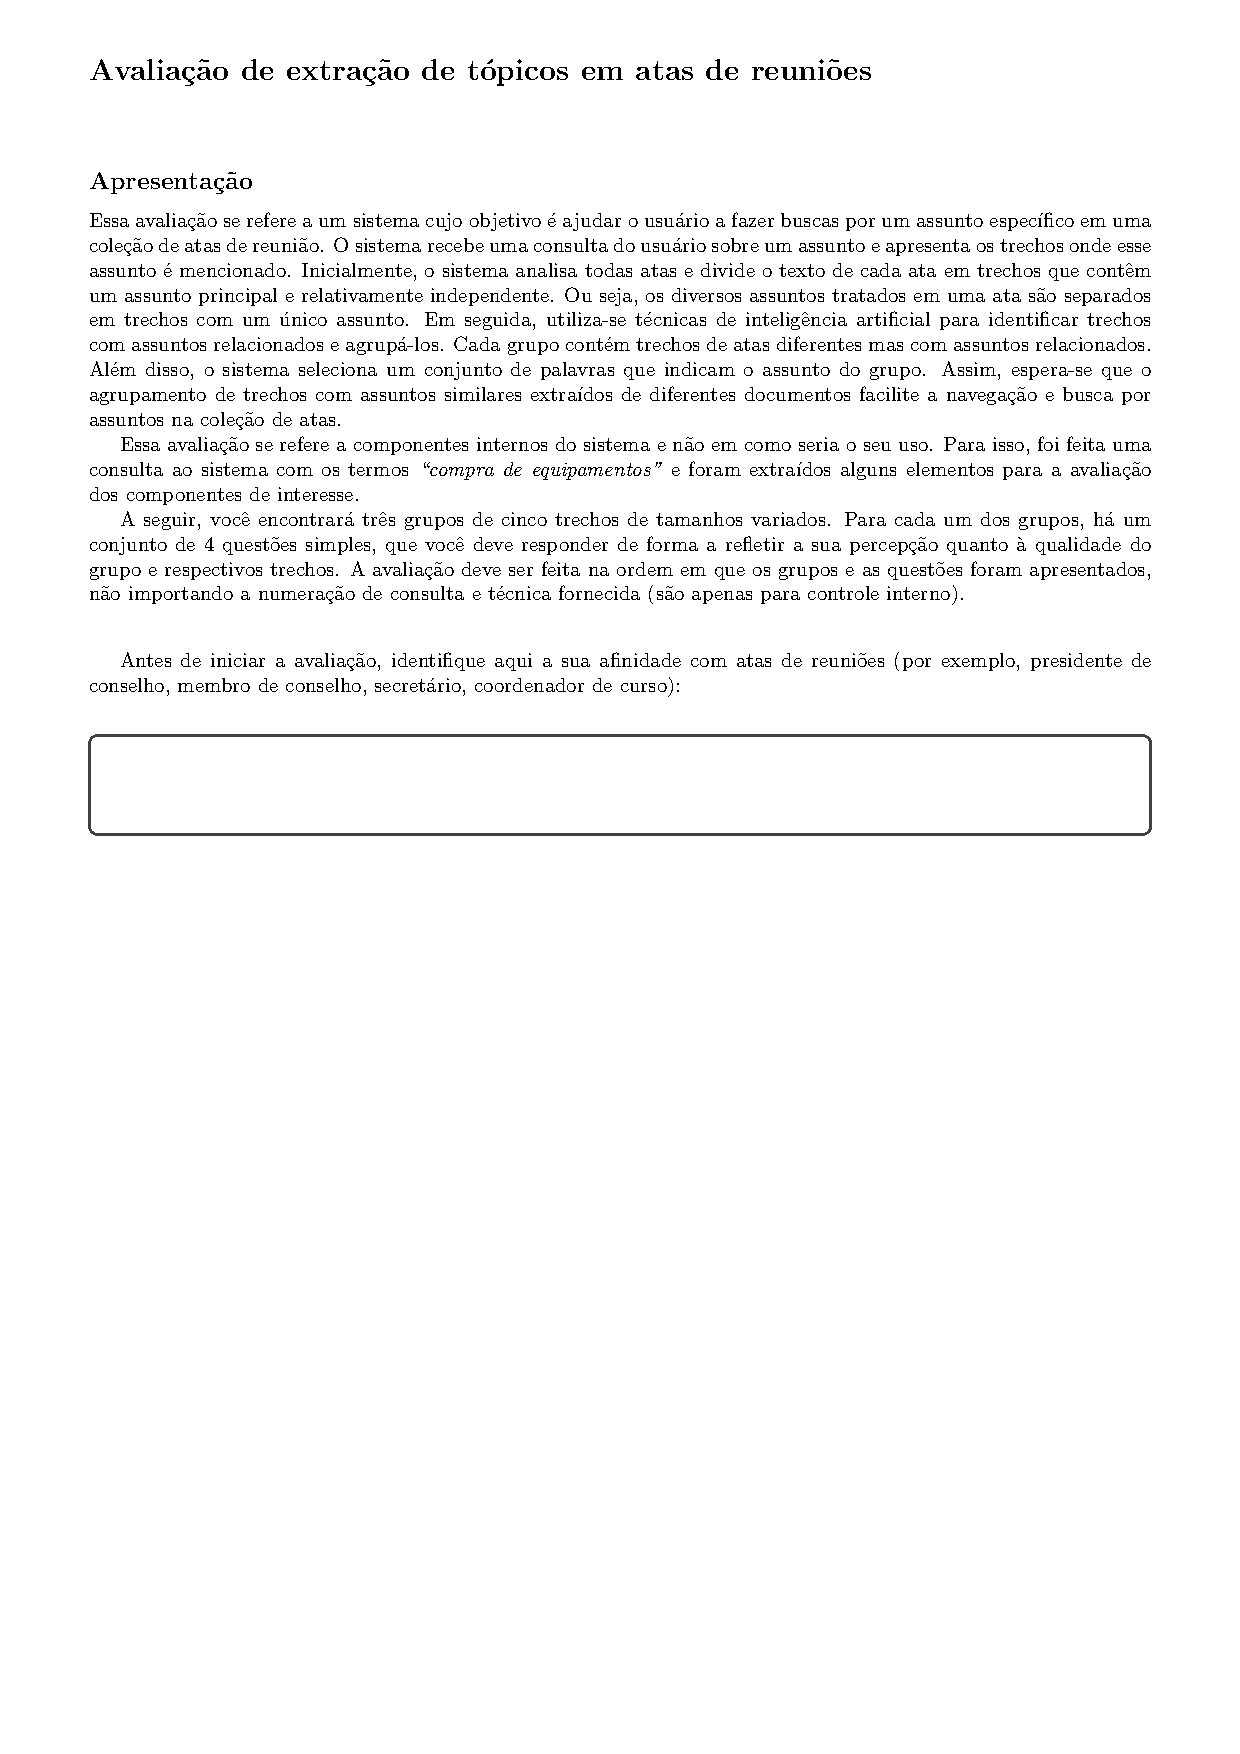
\includegraphics[trim={ 0 60 0 66 },clip,page=1,width=0.8\textwidth]{anexos/avaliacao-sistema/avaliacao-sistema.pdf}

\begin{figure}[h!]
\center
	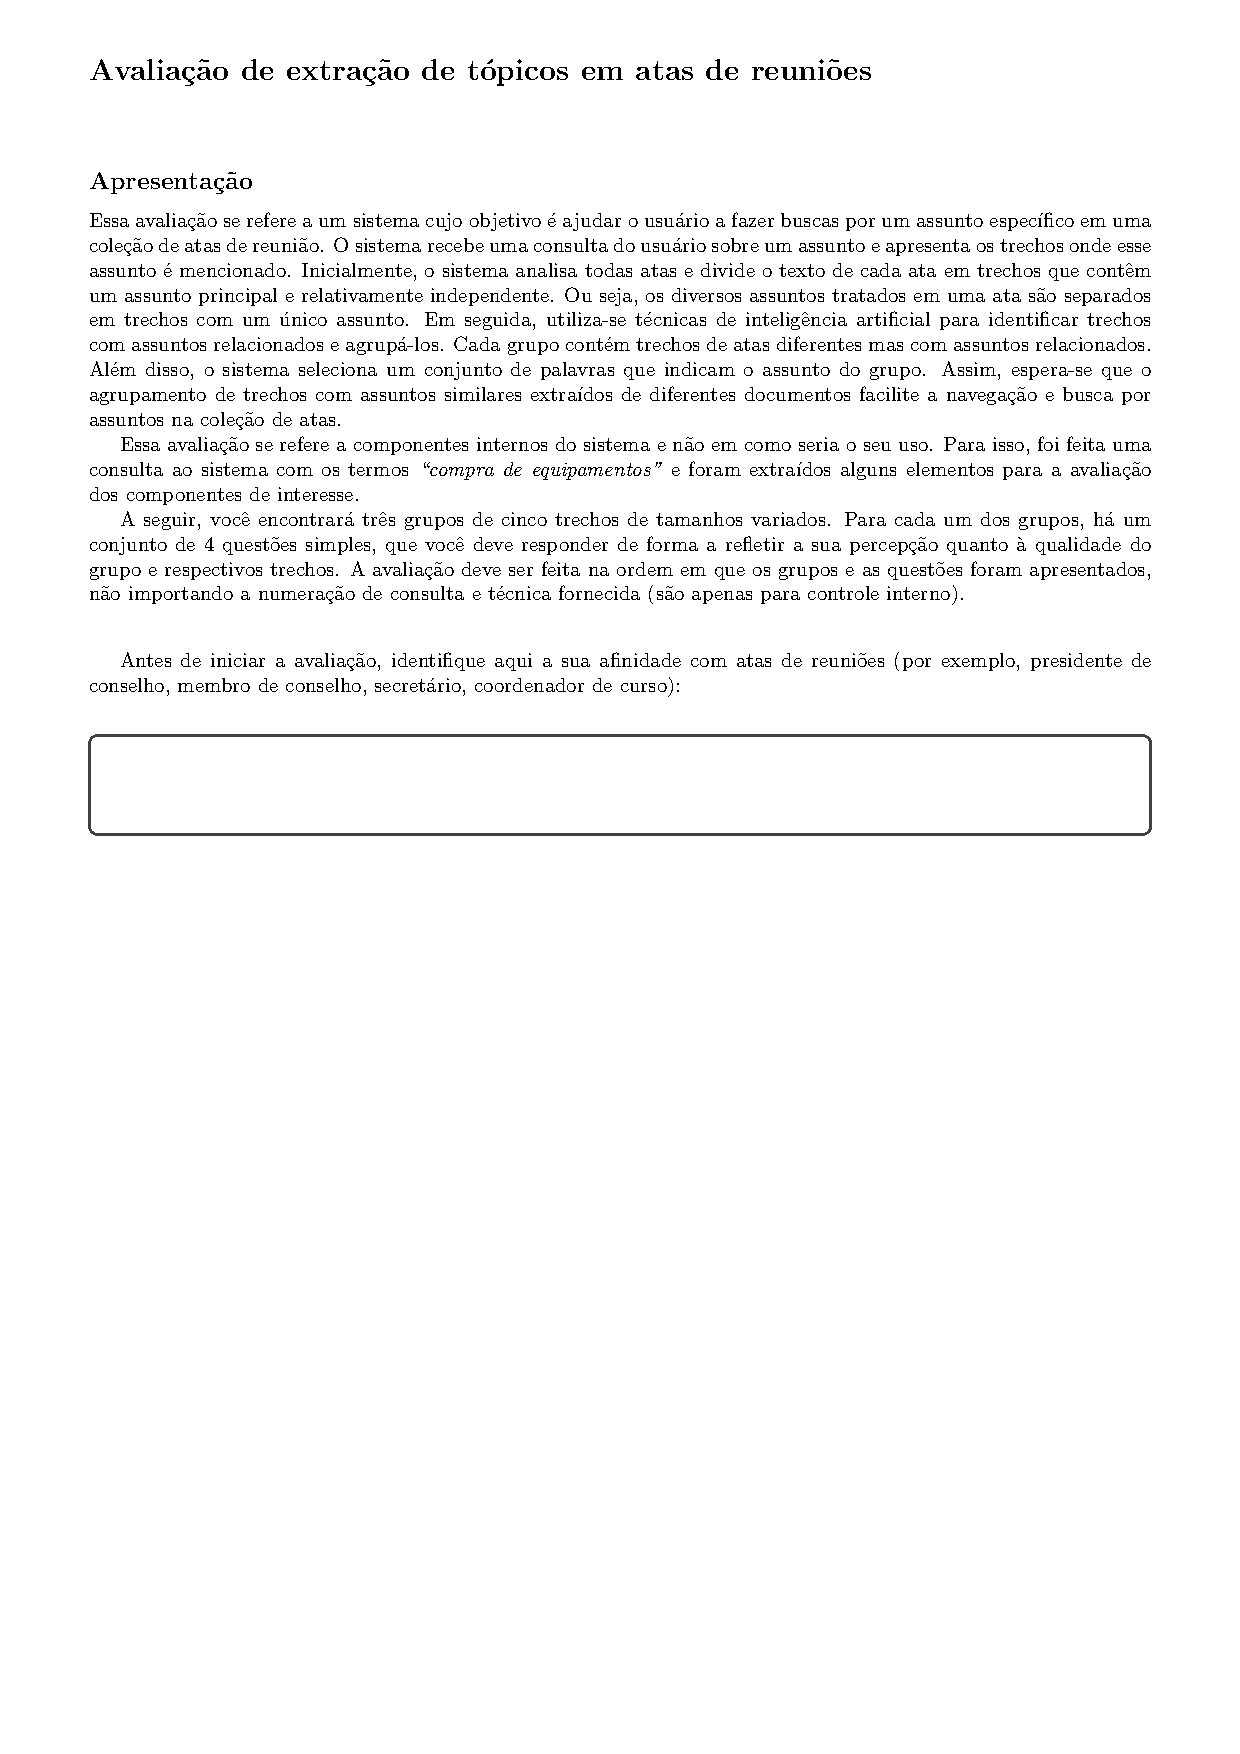
\includegraphics[trim={ 40 0 0 0 }, trim={ 0 60 0 66 }, page=1,width=1.1\textwidth]{anexos/avaliacao-sistema/avaliacao-sistema.pdf}
\end{figure}


\begin{figure}[h!]
\center
	\includegraphics[trim={ 40 0 0 0 }, page=2,width=1.1\textwidth]{anexos/avaliacao-sistema/avaliacao-sistema.pdf}
\end{figure}



\begin{figure}[h!]
\center
	\includegraphics[trim={ 40 0 0 0 }, page=3,width=1.1\textwidth]{anexos/avaliacao-sistema/avaliacao-sistema.pdf}
\end{figure}

\begin{figure}[h!]
\center
	\includegraphics[trim={ 40 0 0 0 }, page=4,width=1.1\textwidth]{anexos/avaliacao-sistema/avaliacao-sistema.pdf}
\end{figure}

\begin{figure}[h!]
\center
	\includegraphics[trim={ 40 0 0 0 }, page=5,width=1.1\textwidth]{anexos/avaliacao-sistema/avaliacao-sistema.pdf}
\end{figure}

\begin{figure}[h!]
\center
	\includegraphics[trim={ 40 0 0 0 }, page=6,width=1.1\textwidth]{anexos/avaliacao-sistema/avaliacao-sistema.pdf}
\end{figure}



\begin{figure}[h!]
\center
	\includegraphics[trim={ 40 0 0 0 }, page=7,width=1.1\textwidth]{anexos/avaliacao-sistema/avaliacao-sistema.pdf}
\end{figure}




\begin{figure}[h!]
\center
	\includegraphics[trim={ 40 0 0 0 }, page=8,width=1.1\textwidth]{anexos/avaliacao-sistema/avaliacao-sistema.pdf}
\end{figure}




\begin{figure}[h!]
\center
	\includegraphics[trim={ 40 0 0 0 }, page=9,width=1.1\textwidth]{anexos/avaliacao-sistema/avaliacao-sistema.pdf}
\end{figure}



\begin{figure}[h!]
\center
	\includegraphics[trim={ 40 0 0 0 }, page=9,width=1.1\textwidth]{anexos/avaliacao-sistema/avaliacao-sistema.pdf}
\end{figure}

\begin{figure}[h!]
\center
	\includegraphics[trim={ 40 0 0 0 }, page=10,width=1.1\textwidth]{anexos/avaliacao-sistema/avaliacao-sistema.pdf}
\end{figure}

\begin{figure}[h!]
\center
	\includegraphics[trim={ 40 0 0 0 }, page=12,width=1.1\textwidth]{anexos/avaliacao-sistema/avaliacao-sistema.pdf}
\end{figure}

\begin{figure}[h!]
\center
	\includegraphics[trim={ 40 0 0 0 }, page=13,width=1.1\textwidth]{anexos/avaliacao-sistema/avaliacao-sistema.pdf}
\end{figure}

\begin{figure}[h!]
\center
	\includegraphics[trim={ 40 0 0 0 }, page=14,width=1.1\textwidth]{anexos/avaliacao-sistema/avaliacao-sistema.pdf}
\end{figure}


